\documentclass[12pt,a4paper]{scrartcl}
\usepackage[utf8]{inputenc}
\usepackage[ngerman]{babel}
\usepackage{amsmath}
\usepackage{amssymb}
\usepackage{tabularx}
\usepackage{graphicx}
\usepackage{color}
\usepackage{hyperref}

\parskip 12pt
\parindent 0pt
\renewcommand{\labelenumi}{\alph{enumi})}
\renewcommand{\labelenumii}{\arabic{enumii})}

\definecolor{darkblue}{rgb}{0,0,.5}
\hypersetup{
  pdftitle={Helix Script},
  pdfauthor={TroY},
  colorlinks=true,
  breaklinks=true,
  linkcolor=black,
  menucolor=black,
  pagecolor=black,
  urlcolor=darkblue
}

% Setzt Zeilenabstand in align-Umgebungen:
\setlength{\jot}{12pt}

\begin{document}

	\begin{center}
		\begin{LARGE}
			\textbf{Helix Script 0.3}
		\end{LARGE}
		
		\textbf{Extract Object Collections 0.1.2}

		\textit{- TroY, März 2008 -} \\
		\textit{\href{http://www.uninformativ.de}{uninformativ.de}}
	\end{center}
	
\bigskip

\tableofcontents

\pagebreak

\section{Einleitung}
Mit dem Helix Script wird es in Art of Illusion möglich, Spiralen auf
einfache Art und Weise an einer beliebigen Kurve entlang zu führen. Da
Bilder mehr als tausend Worte sagen:
\begin{center}
	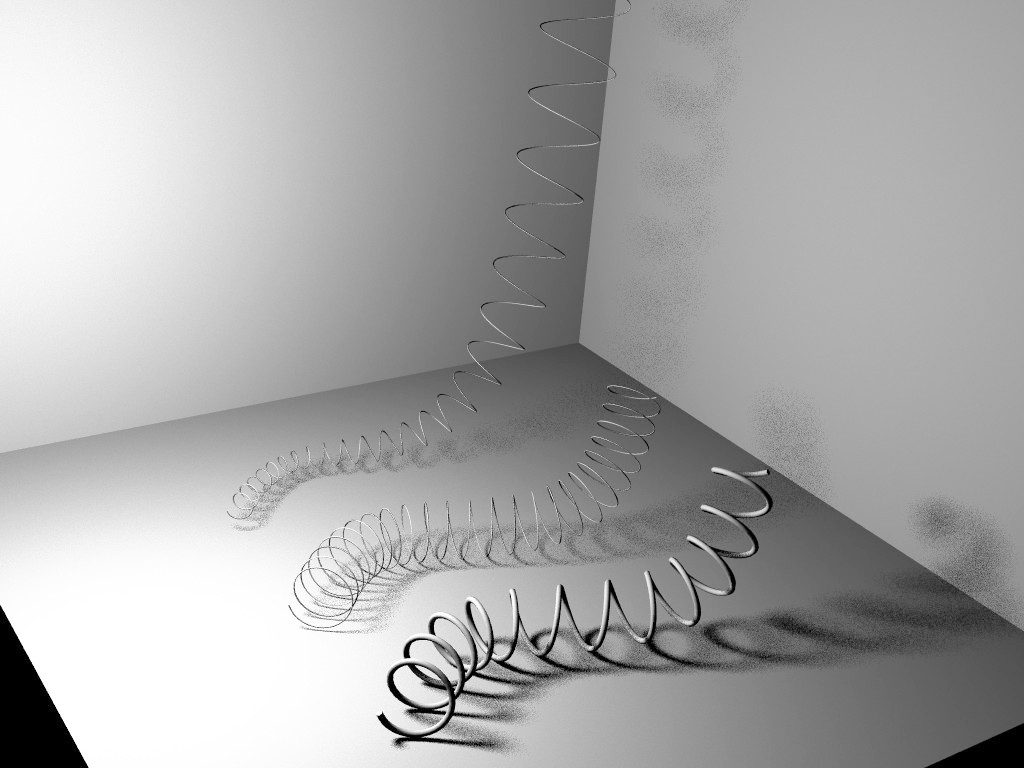
\includegraphics[width=0.75\textwidth]{../pics/presentation-bright.jpg}
\end{center}

Man könnte solche Helices als Telefonkabel, Leitungen für LKW, DNS-Stränge,
ein Ringelschwänzchen für ein Schwein oder was auch immer benutzen.

Wie auf obigem Bild zu sehen ist, kann die Helix in ihrer \emph{Dichte},
\emph{Dicke} und in ihrem \emph{Radius} variiert werden - der Radius
kann außerdem noch \emph{im Verlauf der Spirale} beeinflusst werden.
Das Endprodukt des Scripts kann eine fertige Tube oder eine rohe Kurve
sein, um auf dieser weiterzuarbeiten.

Im Gegensatz zu Version 0.1 gibt es jetzt nur noch einen Weg, eine
Helix zu erstellen: als ein \emph{Scripted Object}. Dadurch bleiben die
Parameter der Spirale die ganze Zeit über editierbar, außerdem wird die
Helix fest mit ihrer Trajektorie\footnote{Dieses Wort macht hier am
meisten Sinn, aber es geht dennoch um normale Kurven - man muss also
nicht das ``trajectory'' Script benutzen.} verheiratet, was die Basis
für die Animation darstellt.

Soll die generierte Curve/Tube als normales Objekt weiterverwendet
werden, so kann dafür jetzt das \emph{Extract Object Collections Tool}
verwendet werden. Dieses ist als separates Script in diesem Paket
enthalten und wird in einem späteren Kapitel genauer behandelt.

\section{Installation}
Die Installation ist sehr einfach:
\begin{itemize}
	\item \texttt{Helix.bsh} kommt in das \texttt{Scripts/Objects} -
	Unterverzeichnis von Art of Illusion
	\item \texttt{ExtractObjectCollections.bsh} kommt in das
	\texttt{Scripts/Tools} - Unterverzeichnis von Art of Illusion
\end{itemize}
Falls AoI während dieses Vorgangs lief, sollte es besser neu gestartet
werden, bevor man versucht, die Scripte zu verwenden.

\section{Erstellen einer Helix}
Im Regelfall muss zuerst eine Trajektorie als normale Kurve erstellt
werden. Danach fügt man über ``Tools'', ``Created Scripted Object''
ein neues ``Scripted Object'' in die Szene ein. Es erscheint ein
neues Fenster, in welchem der Name für das Script eingegeben und das
Script selbst ausgewählt werden muss (namens ``Helix''). Das nächste
Fenster zeigt das Script auch schon an - das ist die Stelle, an der die
Parameter für die Spirale gesetzt werden:
\begin{center}
	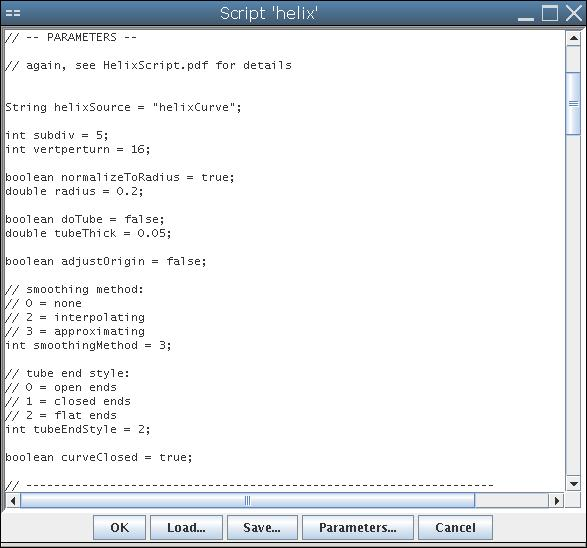
\includegraphics[width=0.5\textwidth]{../pics/createSO.jpg}
\end{center}
Wichtig ist hier der Parameter \texttt{helixSource}: Das ist der Name
des Objektes, welches als Trajektorie genutzt werden soll. Der
Default-Wert ist hier ``helixCurve'' - es muss also entweder der Name
hier im Script geändert oder das Objekt ansich umbenannt werden, damit
es vom Script gefunden werden kann. Klar ist, dass jede Trajektorie
einen eigenen Namen tragen muss, falls mehrere Helices gebaut werden
sollen.

Um den Code nach der Zeile voller Bindestriche braucht man sich nicht
zu kümmern.

\section{Parameter}
\subsection{Quellobjekt: \texttt{helixSource}}
Wie oben schon erwähnt, muss der Parameter \texttt{helixSource} auf das
Objekt gesetzt werden, welches als Richtkurve fungieren soll. Dadurch
wird der Pfad beschrieben, um welchen sich die Helix windet.

Dieses Objekt muss keine primitive \emph{Curve} sein, sondern kann auch
eine \emph{Tube} oder sogar eine andere \emph{Object Collection} sein.

In Art of Illusion sind Object Collections generische\footnote{Nicht
``generic'' wie in ``Java Generics''. ;)} Container, die eine beliebige
Anzahl an beliebigen Objekten enthalten können. Am häufigsten werden 
einem hier wohl andere Scripted Objects begegnen, aber auch der
\emph{Tree and Plant Designer} generiert solche Objekte.

Das hat folgende Konsequenzen:
\begin{itemize}
	\item Helices können um beliebige Curves herum gebaut werden ...
	\item ... es können stattdessen aber auch Tubes dafür verwendet
		werden. Die erste Idee, die mir dabei einfällt, wäre das 
		\emph{Coil Envelope}-Script als Basis für eine Helix zu benutzen,
		da dieses eine Tube erstellt.\footnote{Eigentlich ist es auch
		ein Scripted Object und daher eine Object Collection, aber es enthält
		nur eine einzelne Tube.}
	\item Es ist möglich, ein Helix Script direkt als Basis für eine weitere
		Helix zu verwenden, ohne vorher aus dem ersten Script die Kurve
		extrahieren zu müssen. Somit können doppelte Helices auf einfache Art
		und Weise erstellt werden.
	\item Es können TaPD-Objekte als Basis genutzt werden, aber hier gibt es
		eine Beschränkung: Das Helix Script nutzt die allererste Curve, die es
		in einer Object Collection findet. In den meisten Fällen wird das der
		``Stamm'' der Pflanze sein.
		
		\textbf{Anmerkung:} Man kann das Extraction Tool benutzen, um komplette
		TaPD-Objekte in ihre Einzelteile zu zerlegen. Danach kann man sich die
		gewünsche Tube heraussuchen, um diese eine Helix legen und dann alle
		anderen extrahierten Objekte wieder löschen.
\end{itemize}

Ein Beispiel für eine Kaskadierung zweier Helix Scripts ist in Kapitel 5
beschrieben.

\subsection{Anzahl an Unterteilungen: \texttt{subdiv}}
Bestimmt die Anzahl an Unterteilungen, welche an der Trajektorie vorgenommen
werden bevor die Helix erstellt wird (dies beeinflusst das originale Objekt
nicht, der Vorgang ist nur temporär). Da die Spirale um diese unterteilte Kurve
gebaut wird, kann man damit die \emph{Dichte} beeinflussen: Je mehr Unterteilungen
man hat, desto dichter wird die Helix sein.

Zusätzlich hat die Dichte der Trajektorie selbst einen ähnlichen Einfluss. Wie
man unten sehen kann befinden sich links unten mehr Punkte als rechts oben -
die Helix übernimmt diese Dichte dann:
\begin{center}
	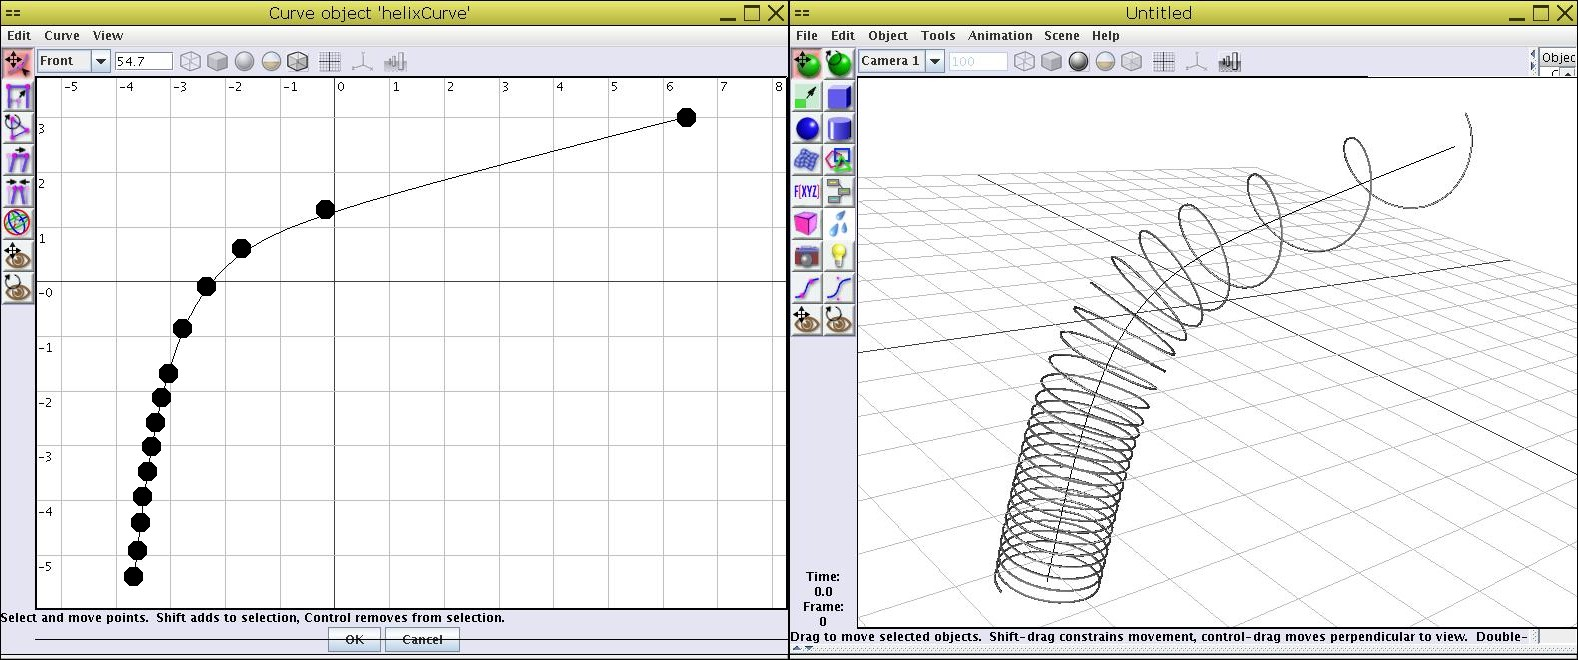
\includegraphics[width=0.75\textwidth]{../pics/dichte-comp-1.jpg}
\end{center}

\textbf{Achtung:} Es dreht sich hier um die Anzahl der
Punkte\textbf{verdoppelungen}! Das heißt also, dass sich beim Wert 6 schon
doppelt so viele Punkte in der unterteilten Richtkurve befinden wie
beim Wert 5. Dementsprechend exponentiell wächst dann natürlich auch
die Berechnungszeit der Helix, es kann bei zu großen Werten also schon
eine Weile dauern.

\subsection{Punkte pro Umdrehung: \texttt{vertperturn}}
Gibt die Anzahl an Punkten pro Umdrehung an. Klar, je mehr Punkte pro
Umdrehung, desto ``runder'' ist das Endergebnis, desto mehr Faces
entstehen aber auch.

\subsection{Radius Normalisierung (\texttt{normalizeToRadius}) und Radius (\texttt{radius})}
Ist die Normalisierung aktiviert, dann wird die Spirale immer genau den 
eingestellten Radius aufweisen. Andernfalls kann der Radius über die
Dichte der Punkte auf der Richtkurve beeinflusst werden - in diesem Falle
ist der Wert \texttt{Radius} nicht mehr in normalen AoI-Einheiten zu
verstehen, sondern eher als grobe Richtlinie, außerdem sollte er dann
mindestens um den Faktor 10 bis 100 größer sein, um einen ähnlich großen
tatsächlichen Radius zu produzieren.

So sieht die Spirale von oben ohne Normalisierung aus:
\begin{center}
	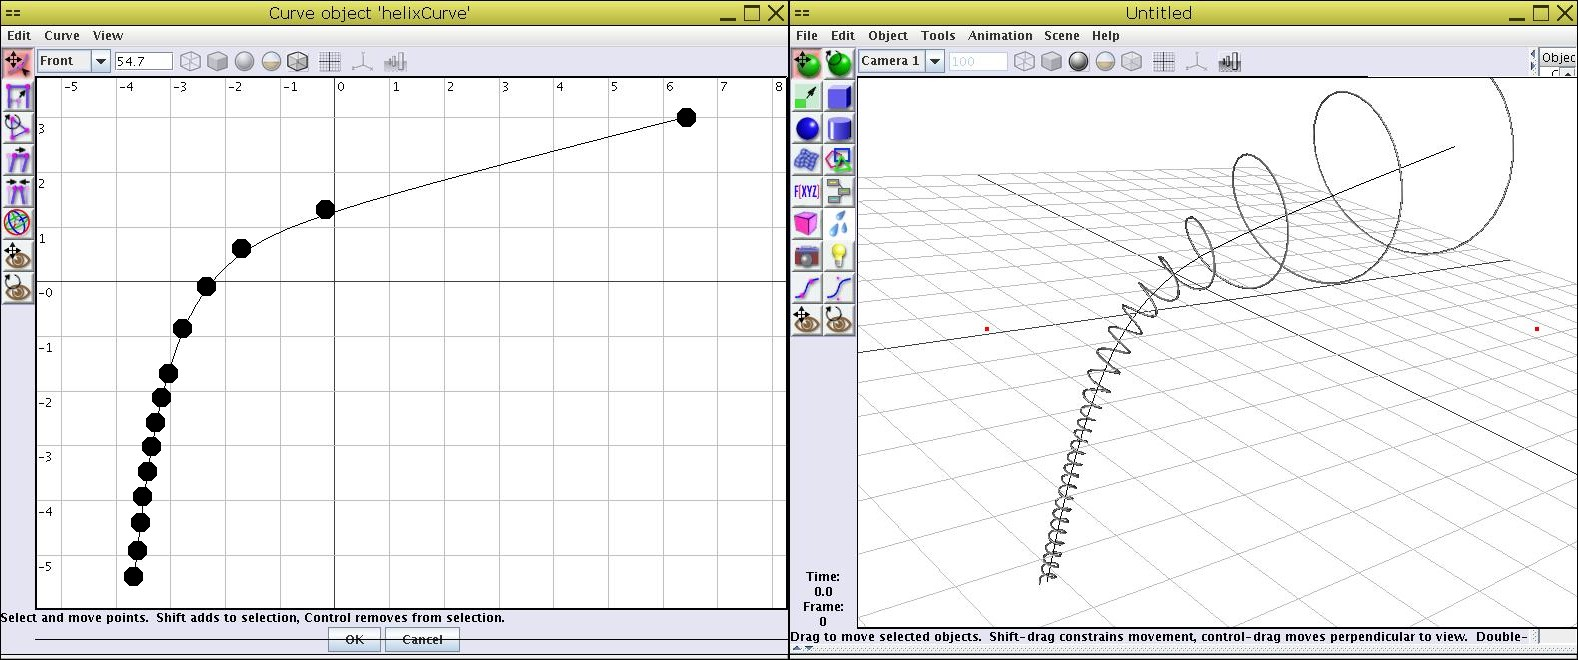
\includegraphics[width=0.75\textwidth]{../pics/dichte-comp-2.jpg}
\end{center}

\subsection{Tube erstellen (\texttt{doTube}) und Röhrendicke (\texttt{tubeThickness})}
Das sind eigentlich selbsterklärende Parameter: Soll das Ergebnis eine
fertige Tube oder nur eine rohe Kurve sein? Wenn es eine Tube sein soll,
wie groß soll deren Dicke dann sein?

\subsection{Dickenanpassung: \texttt{thickTapering}}
Wenn eine Tube erstellt wird und die Radius Normalisierung \emph{deaktiviert}
ist, kann man Dickenanpassung aktivieren. Dann wird abhängig vom aktuellen
Radius der Spirale die Dicke der Röhre auch angepasst.

\pagebreak

Oben ist Dickenanpassung deaktiviert, unten aktiviert:
\begin{center}
	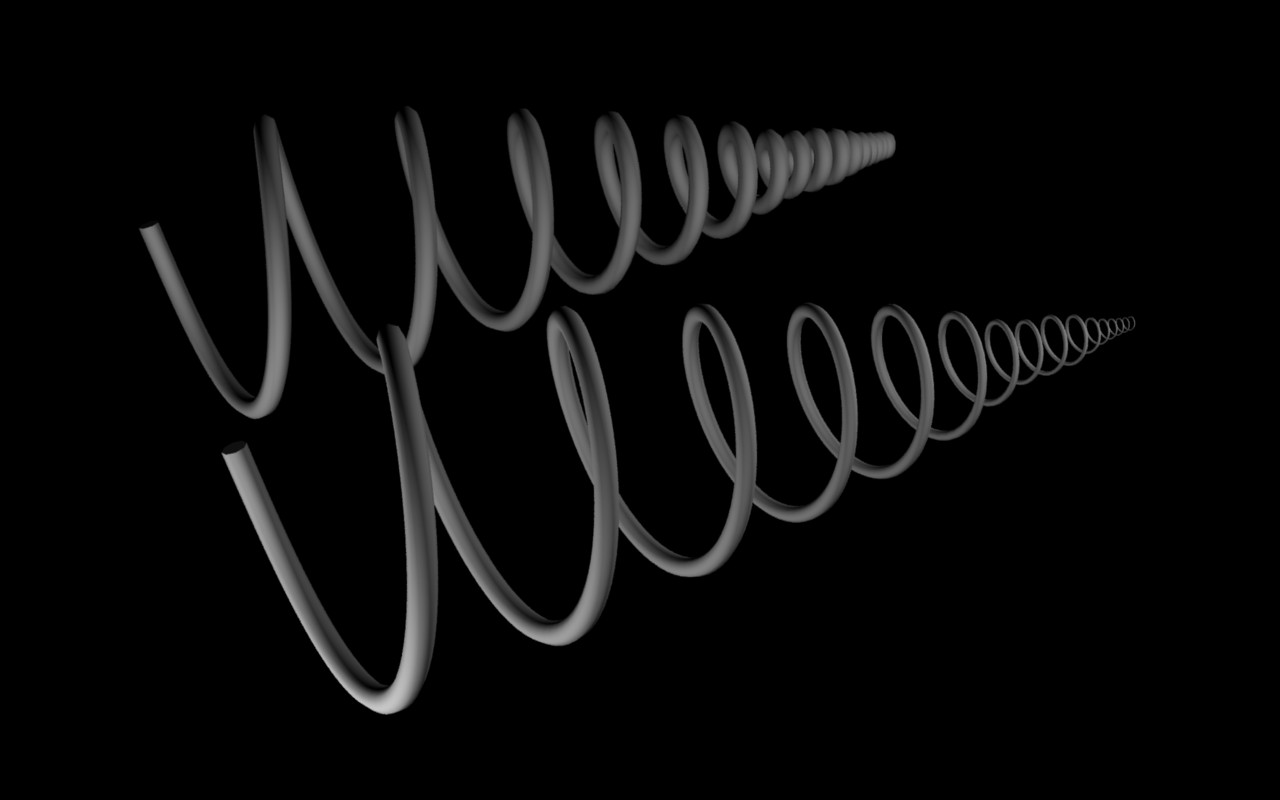
\includegraphics[width=0.75\textwidth]{../pics/thicknessTapering.jpg}
\end{center}

\subsection{Positionsanpassung: \texttt{adjustOrigin}}
Ist dieser Parameter auf \texttt{true} gesetzt, so passt sich das Script
der Position und Rotation des Basisobjektes an - die Helix wird also
immer genau dort platziert sein, wo sich auch ihre Richtkurve befindet.

Steht der Wert auf \texttt{false}, dann platziert sich das Script
initial am Koordinatenurpsrung (0, 0, 0) und kann danach frei verschoben
werden.

Daraus leitet sich auch der Grund ab, wieso hier die Standardeinstellung
\texttt{false} ist: Bei aktivierter Justierung ist das Script nicht
frei verschiebbar, sondern wird immer wieder zur Kurve zurückschnappen.

\subsection{Gewöhnliche Parameter: \texttt{smoothingMethod}, \texttt{tubeEndStyle}, \texttt{curveClosed}}
Diese beiden Werte bestimmen - wie auch bei jeder anderen Curve bzw.
bei jeder anderen Tube -, wie das Objekt ``gesmoothed'' werden soll
und, falls eine Tube erstellt werden soll, den Typ der Enden dieser Röhre.
Wird dagegen nur eine Curve erstellt, gibt ``curveClosed'' an, ob Anfang
und Ende der Curve verbunden werden sollen.

\pagebreak

Die numerischen Werte, die gesetzt werden können, und ihre Bedeutungen:

\underline{\texttt{smoothingMethod}}
\begin{itemize}
	\item 0 = Kein Smoothing
	\item 2 = Interpolation
	\item 3 = Annäherung
\end{itemize}

\underline{\texttt{tubeEndStyle}}
\begin{itemize}
	\item 0 = Offene Enden und damit eine hohle Röhre
	\item 1 = Miteinander verbundene Enden (entspricht also
		\texttt{curveClosed = true} bei einer Curve)
	\item 2 = Flache Enden, nicht verbunden
\end{itemize}

\subsection{Fehlerkorrektur (\texttt{glitchCorrection})}
Leider passieren in bestimmten Situationen hin und wieder noch Fehler. Einerseits
liegt das an der beschränkten Rechengenauigkeit heutiger Computer, andererseits
ist das auch ein klarer Schwachpunkt in der Berechnungsroutine für die Helix.

Bei der linken Helix ist \texttt{glitchCorrection} auf 1 gesetzt, bei der
anderen auf -1. Eigentlich ist \texttt{glitchCorrection} ein Faktor, der das
Vorzeichen eines Winkels darstellt, weshalb hier nur Werte von 1 oder -1 Sinn
machen.
\begin{center}
	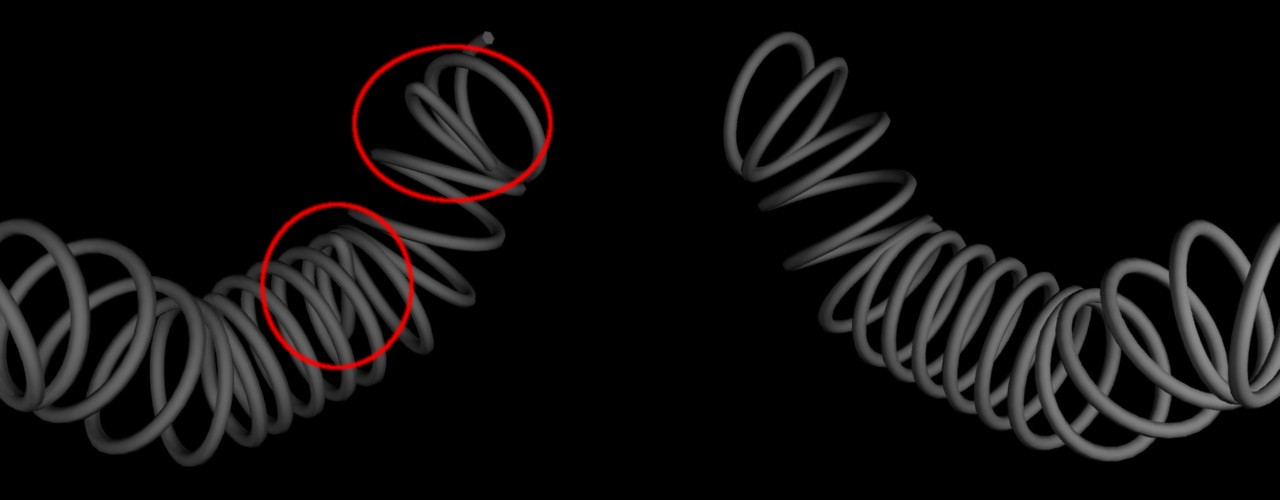
\includegraphics[width=0.75\textwidth]{../pics/glitchCorr-edit.jpg}
\end{center}

Wie man sieht treten links noch zwei Fehler auf, die rechts dann korrigiert
sind.

\subsection{Versatz der Spirale (\texttt{spiralOffset})}
Dieser Parameter bestimmt den Winkel, nachdem die Spirale starten soll. Ein
Wert von ``180.0'' bewirkt beispielsweise, dass die Spirale einmal um die
Richtkurve ``geflippt'' ist.

\section{Animation von Helices}
Seit Art of Illusion 2.6 ist es möglich, primitive Curves und Tubes zu animieren.
Das funktioniert genauso wie bei anderen Objekten, wenn man also auf Probleme
stößt, sollte man zuerst einen Blick in das
\href{http://www.uninformativ.de/tutorials/Vidiot/AoI_Manual_2_5_ger.zip}{Deutsche Handbuch}
werfen.

Wie auch immer, hier ein kurzes Beispiel.
\begin{itemize}
	\item Zuerst muss die Trajektorie in einen Actor konvertiert werden -
		das heißt, dass man nicht mehr in der Lage sein wird, Punkte
		hinzuzufügen oder zu löschen, dafür kann man der Kurve jetzt ``Poses''
		zuweisen. Über ``Object'', ``Convert to Actor'' führt man diese
		Konvertierung durch.
	\item Doppelklick auf die Kurve, um ihr ein paar Posen zu spendieren.
	\item Hinzufügen eines \emph{Pose Track}s: Kurve auswählen und dann
		``Animation'', ``Add Track to Selected Object'', ``Pose'' wählen.
	\item Ein paar Keyframes hinzufügen.
	\item Hinzufügen eines Helix Scriptes, dessen Parameter \texttt{helixSource}
		auf den Namen der Actor-Curve gesetzt wird.
	\item Bewege den Zeitschieber, um zu sehen, wie sich die Spirale biegt.
\end{itemize}

\begin{center}
	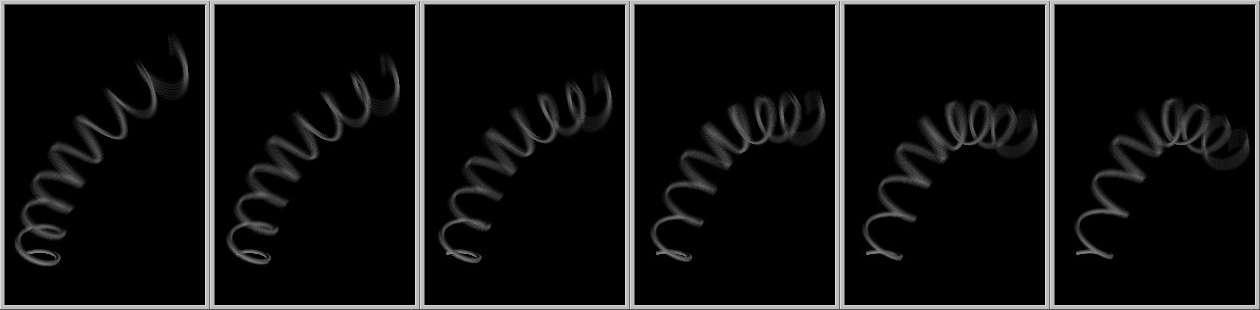
\includegraphics[width=0.75\textwidth]{../pics/helixAni.jpg}
\end{center}

Wenn solche Animationen gerendert werden, ist \emph{Motion Blur} ein sehr zu
empfehlendes Feature.

\subsection{Benutzung von dynamischen Parametern in Animationen}
Optional kann man auch einen Pose Track zum Script selbst hinzufügen. Dadurch
wird es möglich, manche Parameter mit der Zeit verändern zu können:
\texttt{radius}, \texttt{tubeThick}, \texttt{spiralOffset}
und \texttt{glitchCorrection}.

Das Script schaut, ob dynamische Parameter definiert wurden. Wenn nicht,
verwendet es weiterhin die statischen Werte, die direkt im Script gesetzt
wurden.

Wie man dynamische Parameter hinzufügt:
\begin{itemize}
	\item Doppelklick auf das Script, um das Editor Fenster anzuzeigen
	\item Klick auf ``Parameters...''
	\item Klick auf ``Add'', wodruch ein neuer Parameter eingeführt wird
	\item Benenne diesen Parameter genauso wie im Script selbst: ``radius'',
		``tubeThick'' oder was auch immer (Groß-/Kleinschreibung beachten)
	\item Eingabe eines Default-Wertes und dann ein Klick auf ``OK''
	\item Nun kann man den Pose-Track zum Script hinzufügen. Wird dann ein
		Keyframe erstellt, kann man doppelt darauf klicken und dort für diesen
		Zeitpunkt die gerade eben erstellten Parameter editieren.
\end{itemize}

Der Parameter \texttt{glitchCorrection} wird allerdings leicht anders übersetzt:
Da hier nur die beiden Werte 1 oder -1 erlaubt sind, wird nur der genaue Wert
``1.0'' zu ``1'' übersetzt, alles andere dagegen zu ``-1''.

\section{Kaskadierung von Helices}
Hier ein konkretes Beispiel, um zwei Helix-Scripts hintereinander
zu schalten.

\begin{enumerate}
	\item Erstellen einer beliebigen Richtkurve - diese am besten
		gleich ``helixCurve'' nennen.
	\item Wie oben beschrieben ein neues Helix-Script als
		\emph{Scripted Object} in die Szene bringen. Als Namen des Scriptes 
		gebe man hier ``helixScript1'' an. Da wir die Kurve ansich
		gleich richtig benannt haben, entfällt dieser Umbenennungsschritt
		nun. 
	\item Manuell Feineinstellungen vornehmen im Bezug auf Subdivisions
		und Radius, sodass diese erste Helix es leicht zulässt, eine
		zweite auf ihr zu bauen (im Klartext also nicht alles zu eng
		aneinanderfriemeln).
	\item Einfügen eines zweiten \emph{Scripted Object}'s, natürlich
		wieder ein Helix-Script. Dieses bekommt nun als Wert für
		\texttt{helixSource} den Namen ``helixScript1'' gesetzt und
		damit wird dieses zweite Script angewiesen, direkt den Output
		des ersten zu verwenden.
\end{enumerate}

Ein mögliches Ergebnis einer solchen Kaskadierung:
\begin{center}
	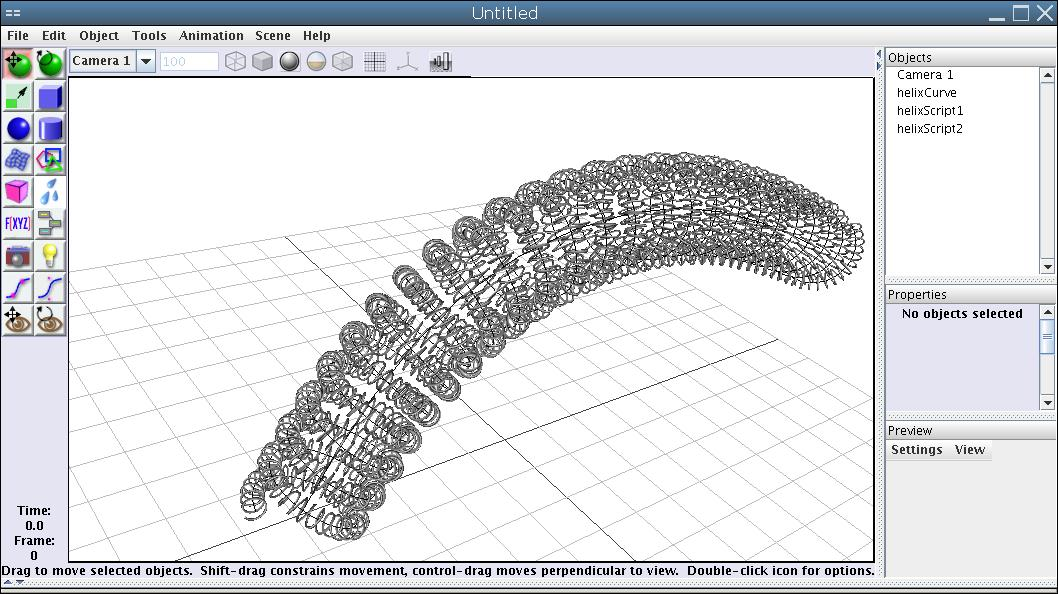
\includegraphics[width=0.75\textwidth]{../pics/doubleHelix.jpg}
\end{center}

\section{Extraktion von Objekten aus Object Collections}
Mittels des Scripts \texttt{ExtractObjectCollections.bsh} können
allgemein alle Objekte aus einer Collection extrahiert werden. Ob
diese Collection ein Scripted Object ist oder etwas ganz anderes,
spielt auch hier keine Rolle.

Um eine solche Extraktion durchzuführen, muss man zuerst alle zu
extrahierenden Objekte in der Liste auswählen (Helix-Scripts,
TaPD-Objekte oder was auch immer), es können also auch mehrere auf
einen Schlag sein. Danach wählt man ``Tools'', ``Scripts'' und dort
``ExtractObjectCollections''. Hat man ungültige Objekte markiert gehabt,
wird man darüber informiert, aber es werden so viele Objekte wie
möglich extrahiert.

Diese werden dann automatisch gruppiert und entsprechend ihres
Objekttyps benannt, also beispielsweise ``Sphere 1'', ``Sphere 2'',
``Tube 1'', ``Tube 2'' und so weiter.

Alle extrahierten Objekte werden sich an derselben Stelle im Koordinatensystem
befinden wie das Ursprungsobjekt, außerdem weisen sie dieselbe Rotation
auf. Texturen und Materialien werden mitkopiert - auch falls sie noch nicht
in der Szene enthalten sind (was beim Tree and Plant Designer der Fall
ist).

\section{Changelog}
\subsection{Helix}
\underline{0.3}
\begin{itemize}
	\item Fehlerkorrektur hinzugefügt
	\item Bereit für Animation (akzeptiert nun Actors und extrahiert daraus
		die Curve/Tube)
	\item Dynamische Parameter: \texttt{radius}, \texttt{tubeThick},
		\texttt{spiralOffset} und \texttt{glitchCorrection}
	\item Dickenanpassung eingeführt
\end{itemize}
\underline{0.2}
\begin{itemize}
	\item ``Tool''-Version entfernt
	\item Auch Tubes werden als Input akzeptiert
	\item Ebenso beliebige Object Collections - hieraus wird die erste
		Instanz einer Curve (und damit auch einer Tube) genommen
	\item Auf Wunsch Anpassung der Position und Rotation der Helix
		an das Mutterobjekt
	\item Einführung der Parameter \texttt{smoothingMethod},
		\texttt{tubeEndStyle} und \texttt{curveClosed}
\end{itemize}

\subsection{Extract Object Collections}
\underline{0.1.2}
\begin{itemize}
	\item Verallgemeinerung auf beliebige Collections und nicht nur
		Scripted Objects
	\item Texturen und Materialien werden jetzt von den im Container
		enthaltenen Objekten kopiert und nicht mehr vom Container selbst
		(war für korrekten Export von TaPD-Objekten nötig)
	\item Texturen und Materialien, die extrahiert und noch nicht in der
		Szene enthalten sind, werden in diese eingefügt
\end{itemize}

\end{document}
